% -*- mode: latex; mode: auto-fill; coding: utf-8; -*-

\section{The Surgical Procedure}
\label{sec:surgical_procedure}
% The learning process
To gain fundamental knowledge on how the surgical procedure is
performed in real life, the following section will explain each step
involved. This section is based on an interview with Professor,
dr. odont. Søren Schou, Aarhus University, who carefully took his time
to explain the procedure in detail.  \\

% Explain briefly the four scenarios
First of all when it comes to patients with wisdom tooth compilations,
there are not two of a kind, but basically all complications can be
divided into four scenarios. Within each scenario the location of the
tooth can vary but the approach used to remove it is the same. The
four scenarios are illustrated in figure
\vref{fig:wisdom_tooth_scenarios}. The different scenarios require
slightly different approaches when it comes to fragmenting the
tooth. The following steps are carried out in each of the four
scenarios. \\


% \begin{figure}
%   \centering
%   \includegraphics[width=6cm]{./images/problem_domain_surgery_four_tooth_positions.png}
% \caption{The four basic scenarios showing how the wisdom tooth can be
%   located in the jaw.}
% \label{fig:wisdom_tooth_scenarios}
% \end{figure}

\begin{figure}[h]
    \centering
    \subfloat[Angular]{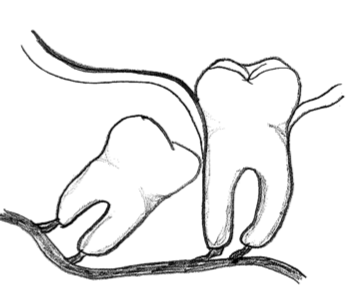
\includegraphics[width=50mm]{./images/problem_domain_surgery_tooth_0.png}}
  \hspace{0.5cm}
    \centering
    \subfloat[Partial Eruption]{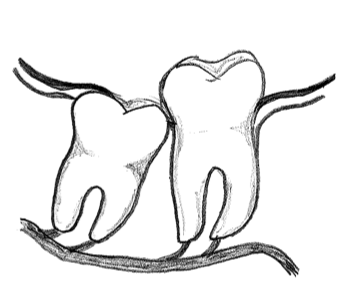
\includegraphics[width=50mm]{./images/problem_domain_surgery_tooth_1.png}}
  \newline
    \centering
    \subfloat[Horizontal]{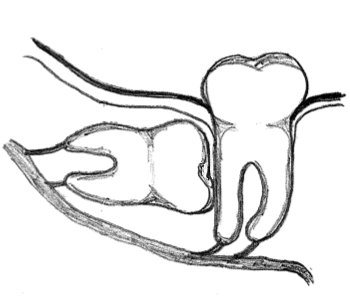
\includegraphics[width=50mm]{./images/problem_domain_surgery_tooth_2.png}}
  \hspace{0.5cm}
    \centering
    \subfloat[Vertical]{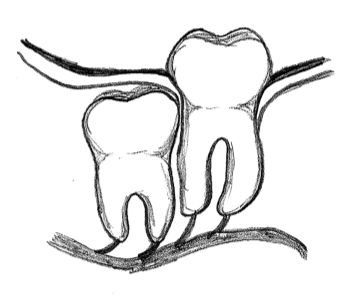
\includegraphics[width=50mm]{./images/problem_domain_surgery_tooth_3.png}}
\caption{The four basic scenarios showing how the wisdom tooth can be
  located in the jaw.}
\label{fig:wisdom_tooth_scenarios}
\end{figure}


As a preoperative task
the dentist carefully examines x-ray images of the wisdom tooth to determine
the risk of nerve damage. It is crucial that the nerves are left
undamaged since this can lead to complete and permanent numbness of
the tongue and lip.


\subsection*{Anaesthesia}
% local anaesthesia to the nerves in the jaw
The surgical procedure can be performed under local anaesthesia,
leaving the patient conscious during the entire operation. The local
anaesthesia is carefully injected directly into the nerves located on
the inside of the jaw,
making the tongue, part of the lip and the wisdom tooth numb. The
anaesthesia substance contains adrenaline which contracts the blood
from the blood vessels, hereby minimizing the bleeding from the wound.
% pinch to check anaesthesia 
Shortly after the anaesthetic injection, the dentist
pinches the surrounding tissue to ensure the area is numb. 


\subsection*{Incision}
% using scalp to perform the tissue cut
The soft tissue surrounding the wisdom tooth, on the outside of the
jaw, needs to be loosened to expose the tooth. 
% always on the outside of the jawbone
The cut starts from the back of the jaw and is carefully placed along the
outside of the first and second molar, illustrated as the red line in
figure \vref{fig:incision_cut}. The yellow dot is where the wisdom
tooth is located, currently covered by soft tissue. It is crucial not
to damage the nerve located on the inside of the jaw, therefore
the incision is always performed on the outside of the
molars.    
% Suction
The cut is made slowly while any blood from the wound is sucked away
with a small tube to keep visibility high and to prevent it from
running down the patients throat. 
%
When the incision has been made, the soft tissue can be pulled to the side hereby
revealing the wisdom tooth and part of the roots of the first and
second molar. 
% the wisdom tooth located down the jaw. 
Often the wisdom tooth is located deep down the jawbone so only the crown
of the tooth is visible when the soft tissue has been removed.

\begin{figure}
  \centering
  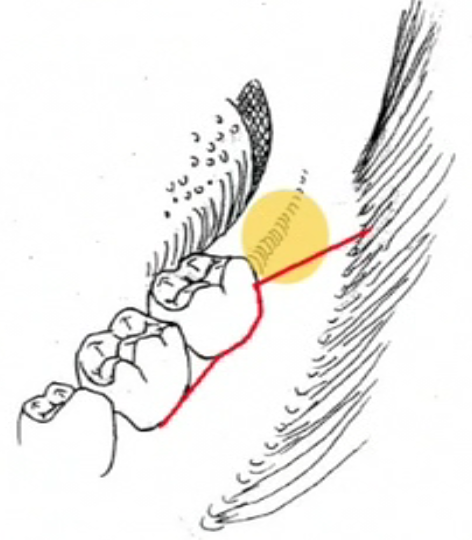
\includegraphics[width=4cm]{./images/problem_domain_surgery_incision.png}
\caption{The red line illustrates where to place the incision. \textdagger}
\label{fig:incision_cut}
\end{figure}

\subsection*{Bone Removal}
Now that the soft tissue is removed the next step is to remove the
surrounding jawbone. This is done using a drill on the outside of the
jaw as illustrated with the red line on figure
\vref{fig:bone_removal}. Drilling away the surrounding jawbone will
expose the wisdom tooth down below its crown. When drilling, the point
of contact between drill and jawbone, is constantly cooled with 
water to prevent the nearby soft tissue from heating up potentially
causing damage.

\begin{figure}
  \centering
  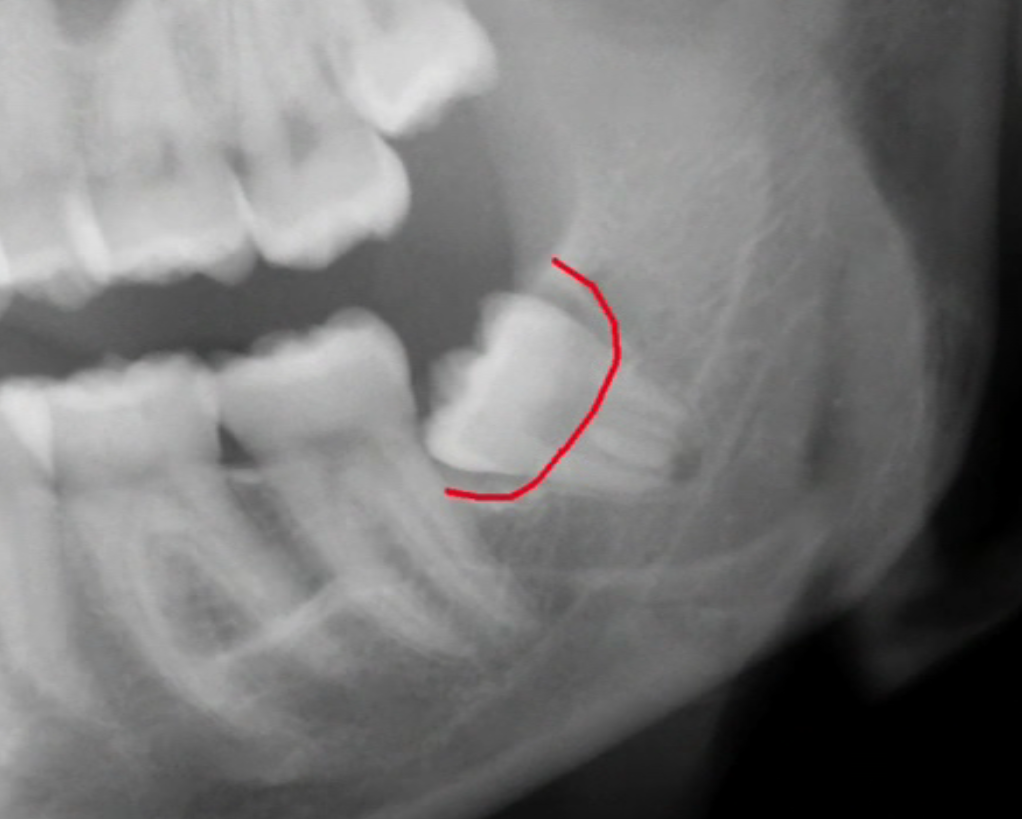
\includegraphics[width=6cm]{./images/problem_domain_surgery_bone_removal_xray.png}
\caption{The red line illustrates where the jawbone must be drilled
  away. \textdagger}
\label{fig:bone_removal}
\end{figure}

\subsection*{Drilling a Groove}
Now that the wisdom tooth has been exposed from both the surrounding
tissue and jawbone, the dentist can move on and prepare a controlled
fragmentation of the tooth. The fragmentation must carefully separate
the crown of the tooth from its roots as illustrated by the red line
in figure \vref{fig:groove_line}. A straight groove is drilled along
the red line. The groove is approximately 5 millimeters deep, or one
third of the tooth, and located right below the crown. 

\begin{figure}
  \centering
  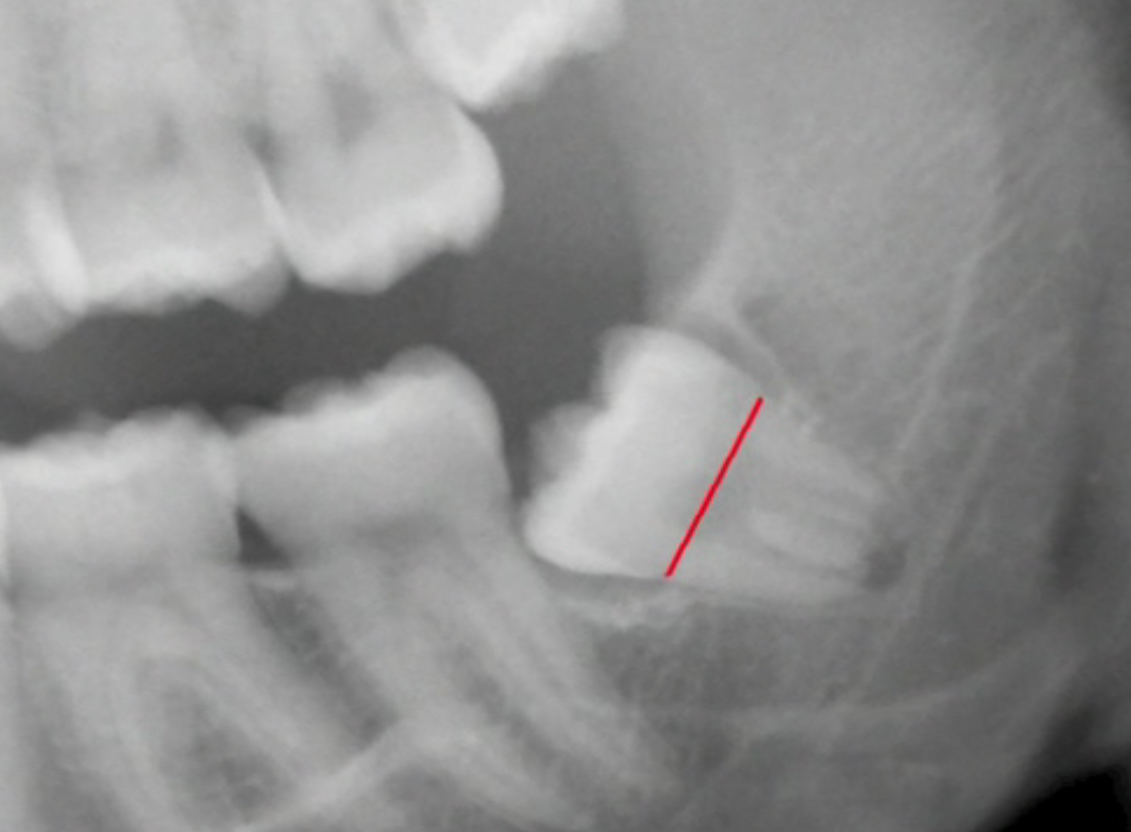
\includegraphics[width=6cm]{./images/problem_domain_surgery_fragmentation_line.png}
\caption{The red line illustrates where the groove should be drilled. \textdagger}
\label{fig:groove_line}
\end{figure}

The dentist always tries to avoid drilling down the enamel on the
crown of the tooth, because it is so hard that the drill will be worn
down too fast.  

\subsection*{Fragmentation}
A special tool known as an \defit{elevator}, illustrated in figure \vref{fig:elevator},
is now inserted into the groove and twisted to separate the crown of
the tooth from its roots. Sometimes, due to the location of the wisdom
tooth, it is necessary to perform further fragmentation to either the
crown or the roots. 

\begin{figure}
  \centering
  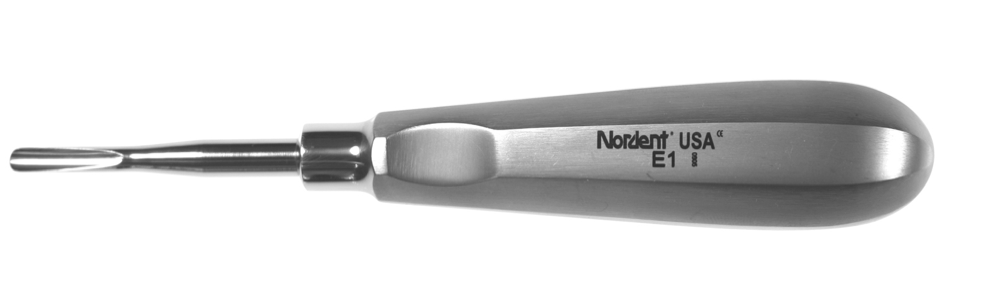
\includegraphics[width=8cm]{./images/problem_domain_surgery_elevator.png}
\caption{Dental tool known as an elevator. \textdagger}
\label{fig:elevator}
\end{figure}


\subsection*{Fracture Removal}
Now that the tooth has been fragmented the individual parts must be removed carefully.
It is very important to make sure all of the fragments are
removed properly. If a small piece is left behind it can cause
complications such as wound infections. 
%
Usually wisdom teeth are removed only if they cause some sort of
complications. A common complication is when other teeth prevent the natural
development, often causing an small infection around the wisdom
tooth. The infected tissue must be removed from the wound as well.      

\subsection*{Smooth Off the Rough Edges}
The dentist has to smooth off the rough edges in the jawbone to
prevent complications with the soft tissue surrounding it.
The crater from where the wisdom tooth was located, must be cleaned
thoroughly with water to wash out every tiny bit of bone from the
drilling. 

\subsection*{Stitching the Wound}
The last step in the surgical procedure is to stitch the wound together. Usually two
stitches is enough but this depends on the size of the
wound. When the stitching is done a small cloth is inserted in the
cheek to absorb any remaining blood. The surgical procedure is now
done.

\section{Simulator}
\label{sec:simulator}
% What is a simulator? (real-time, high-performance workstation)
In context of computer science a simulation is a computational model
that approximates a real phenomenon or procedure. A simulation defines
rules of behaviour reflecting those appearing in the real world. The
results produced by a simulator can be used for evaluation or
prediction of the phenomenon or procedure simulated.  
%
Challenges arise due to the almost unlimited complexity of any real world
phenomena no matter how simple it seems.
Specific parts of the phenomenon being
simulated must be prioritised, but even then only a certain level of detail
can be computed. 
%
If time and computational resources was no issue, designing a
model that strictly represents solid objects by the smallest unit
possible, would be a solution. 
However intuition tells us that it is probably impossible to represent and 
simulate the physical laws for such small units. Let us consider atoms
as the basic unit of matter, the nucleus diameter of an atom is about $10^{-15}$
meter. Even for a small object like a tooth the number of atoms needed
to represent it would be in billions, easily exceeding the computer
resources available. A discrete method must be used in order to
facilitate computation of the problem domain. 


\subsection{Real-time}
\label{sec:real-time}
It is crucial that the simulator gives the impression of a surgical
procedure performed in real-time. 
% Real-time
The concept of simulated real-time can be considered from two
different perspectives. One way is to measure real-time as the speed
of average sensory perception. By measuring real-time this way we consider 
how fast the system is responding to an event such as user
interaction. In this sense real-time is more of an illusion where
users should perceive the simulation feedback at a rate that 
corresponds to the actual scenario in real life. 

\begin{quote}
\defit{"
It doesn’t really matter whether the deformation that the surgeon sees
in the virtual environment is accurate as long as it seems realistic!
Just as important is that the model is robust and shows a consistent
and predictable behavior over time"}
\begin{flushright}
%\hspace{30mm} 
(Morten Bro-Nielsen
\citebook{page~8}{article:bro-nielsen})
\end{flushright}
\end{quote} 

%
Another way of defining real-time is to consider 
the extrapolate of simulation time contra the computation time
used. When simulating a phenomenon time must be discretized into time
steps that represents the difference in time from the current
configuration to the next. If it is possible to compute the next
configuration faster than the time extrapolation it represents we can
predict the behaviour of the phenomenon in real-time. If not we can
pre-compute the behaviour and inspect them at a real-time rate
afterwards, but this rules out real-time interaction which is an
essential part a surgical simulator. \\

To accommodate the demand for real-time execution appropriate solving
techniques must be used. A variety of limitations and approximations
must be taken into account to keep the result plausible. 
When the level of simulation details increases so does the
computational efforts. Making the right decisions in the trade-off
between accuracy and speed is essential. 
%
Each time an
approximation is made the margin of error must be considered to
prevent the final result from ending wide of the mark. 


% Simulation time progresses by the rate of a pre-computed
% time step. The size of the time step is base upon the approximate
% speed of sound waves traveling through the given material. Using this
% definition the simulated time step is representing actual time.  
% %
% If it is possible to compute the simulated time step faster than
% the actual time it represents the simulation is executable in
% real-time.
%

% %
% % As we shall see later some methods used when predicting the next
% % configuration introduces limitations on how fast time exploration can
% % be done.
% %
% When the level of simulation details increases so does the
% computational efforts. Making the right decisions in the trade-off
% between accuracy and speed is essential. 
% %
% Each time an
% approximation is made the margin of error must be considered to
% prevent the final result from ending wide of the mark. 


\subsection{Phenomena}
Before designing a model that represents the processes
we would like to simulate, we need to identify the physical
phenomena. 
% Types of material and their properties. (zoom to see atom grid)
It is no surprise that different materials behave very
differently. Dropping a glass vase on the floor would probably break
it while a rubber ball would bounce back without a scratch. What might
be a surprise to some, is the rather complex physical theory behind
this. The answer to why some materials are able to undergo change in shape without
breaking and others are not, lies in the structure of the
molecules. Since representing a material on the level of molecules
would exceed the computational resources, this phenomenon must somehow be
represented on a higher level.  \\

% Energy and elasticity
A rubber ball can deform into an ellipsoid and still return to its
original shape. In physics elasticity is the property that
makes a material deform due to external forces, but still makes it
return to its original shape when the external forces are removed. This
phenomenon requires a model where external forces somehow are transformed into
energy. \\


% Forces applied to a material causes deformation and induces internal stress, 
% the relative amount of the deformation is referred to as strain. 
% There exists a variety of ways
% to represent elasticity but basically it represents the relation
% between stress and strain. Elasticity, stress and strain are
% fundamental physical concepts that must be understood and incorporate
% into the simulation model. \\   

% Homogen vs. non-homogen
A homogeneous material contains only identical molecular structures
and is therefore a pure material with the exact same properties
everywhere. In the real world this is rarely the case, most materials are a
composition of others. A tooth has different layers each
with different material properties. From that perspective modelling
heterogeneous materials would probably be preferable. \\

% Temperature impact on diff. materials 
It is common knowledge that most material properties change as a
result of change in temperature. When steel is heated its strength
decreases, and rubber cooled down to extremely low degrees can shatter
like glass. Decision must be made whether or not to represent this
phenomenon in the simulation model. \\  

% Fragmentation 
When things break in the real world it often happens in a blink of an
eye. A rule of thumb says that a crack propagates through a brittle
material with the speed of sound. Observing the propagation would
require a 
high speed recording of the phenomenon for later replay in slow motion.
Intuition tells us that the crack must have a point of origin. As the
crack propagates through the material it must somehow choose its path
based on the material properties and the external forces acting upon
the material. 



\section{Problem Statement}
\label{sec:problem_statement}

% Define what part of the simulator we will focus on
As already mentioned the surgical procedure of removing a wisdom tooth
involves various steps of cutting tissue, drilling, fracturing dental
material, stitching tissue, etc. Simulating each step requires a
different approach and the use of distinct theory. It is out of scope
of a single master's thesis to handle all of the different step. \\

% would require a tremendous amount of work impracticable
% due to resources available.
%
Considering the relatively limited amount of work published
within the field of fracturing volumetric models in real-time
compared to the other fields of interest, from the various simulation
steps, attention will be focused on solving this particular problem. \\

This thesis deals with simulating the specific parts of the
dental procedure that involves fragmentation of the tooth. Separating the
crown of the tooth from its roots involves estimation of the internal
stress and prediction of crack propagation through a solid material. 
%
The estimation of internal stress will be based on the finite element
method which is a widely accepted method used for structural
analysis. Using the finite element method to conduct real-time
analysis is a fairly new concept developed within recent years. It
has proved to be one of the most precise methods available.
%
The method for predicting the point of origin will be based upon the
theory of maximum principal stress. 
%
To the best of our knowledge the parallel approach of conducting real-time
structural analysis in conjunction with crack detection, based
upon maximum principal stress is new to the field. \\

% Motivate deformation and fracture framework
The main objective in this thesis is to create a framework for
real-time simulations of deformation and crack initialization in solid
objects. 
%
With point of reference in the laws of physics we will
construct a simulation model that strictly complies with relevant
theory. The context of use is simulated surgery, therefore speed
and robustness of the model will be favoured over accuracy.
%
External forces will be applied through a simulated dental tool, similar
to the elevator actually used by dentists. 
%
The stress and strain analysis will be based on 
the theoretical laws of physics and the crack prediction will be based on
the theory of maximum principal stress direction from fracture mechanics. 
%
We will construct a model aimed towards real-time crack detection
based upon analysis of stress and strain behaviour. If the
internal level of stress exceeds a material-specific threshold the
solid object will fracture. Once the point of origin of the crack has
been predicted the determination of the crack surface is not
considered time critical.


% Focusing on how to simulate the
% physical phenomena involved when applying external forces to a solid
% object and how to 


% A criterion of success is not to develop
% a simulation model which strictly complies with the theoretical laws of
% physics, but to achieve plausible results base on relevant theory. Speed
% and stability will be favoured over accuracy due to the demand of
% real-time execution. 

% The main purpose is to provide a
% realistic training facility and not to provide a framework for
% structural engineers. \\


\section{Related Work}
% Related work from Aarhus University
The purpose of solving the particular problem of how to
fracture solid material in real-time, is to establish a theory 
that will bring the development of a complete dental surgical
simulator one step closer to reality. The simulation model presented
in this thesis is base upon the combination of numerous theories and
existing methods. 
%
The following articles presents closely related work and methods
we have derived our simulation model from. \\

% First on real-time deformation using FEM
Morten Bro-Nielsen was among the pioneers
within real-time simulation of deformable models used for simulated
surgery. Morten Bro-Nielsen
\citeabook{article:fast_fem}\citeabook{article:bro-nielsen} presents a 
method base on a Fast Finite Element (FFE) method and linear
elasticity. The interior nodes
are removed from the equations to improve performance. Even though the
interior nodes are excluded from the calculations the predicted
behaviour of the surface nodes are exactly the same a if interior node
was taking into account. \\

% Miller
% Related work within the field of deformable models aimed towards use
% in surgery simulations, has been presented by
Miller et al. \citeabook{article:miller} present an efficient numerical
method for computing soft tissue in real-time, based upon finite
element analysis. Their method is based on total Lagrangian
formulation relating stress and strain to the original configuration. \\

% TLED
Zeike A. Taylor et al. \citeabook{article:tled} present an improved method
based directly upon the work conducted by \citeabook{article:miller}.
The improvements made are primarily on how to solve the finite element
equations in parallel using the GPU hereby gaining a significant
increase in performance. \\

% Real-time
Thomas Sangild Sørensen and Jesper Mosegaard presents methods on
how surgical simulations can accelerate deformable models through
the parallel nature of the GPU \citeabook{article:gpu_surgery}. They show
that deformable models based on the spring-mass or finite element
method can be implemented using parallel programming, hereby gaining a
significant increase in performance. \\


% Fracture
Depending on how much the wisdom tooth is developed, fragmentation of
the tooth can be necessary. Teeth are primarily made of a material
called dentin which consists of calcium, phosphorus, and other
mineral salts. Dentin is a very hard and brittle material.
Techniques for simulating fracture initialization and
propagation in brittle materials has been presented by O'Brian
et al. \citeabook{article:brittle_fracture}. The method presented is based on
finite element analysis and aimed towards pre-rendered simulations. \\

% First real-time deformation and fracture of stiff materials
Matthias Müller et al. \citeabook{article:muller} present a method for
real-time deformation and fractures in stiff materials. The method
presented introduces a hybrid approach where the simulation is
alternating between simulating rigid body dynamics and the
continuum model at the point of impact. The fragmentation method used
includes model re-meshing which improves the realism of the crack
surface. \\ 

% Different fracturing methods
A comparison of different fracturing techniques has
been conducted by P. Jäger et al. \citeabook{article:crack_tracking_comparison}. The article
compares four different approaches in terms of standard quality
measures such as efficiency, robustness, stability and computational
cost.\\ 

Besides the closely related work, we have also paid attention to the
following articles and PhD theses presenting methods that could be
used for simulating the other parts of the complete simulator. \\

% Haptic feedback by Thomas Sangild
In relation to handling input the user, here being a surgeon,
must be presented to a device capable of simulating the tools similar
to the ones used in real life. Surgeons are used to manoeuvre tools
freely in three-dimensional space. An ordinary computer 
mouse has only two degrees of freedom which makes it unfit. Instead of
conventional user input like those of a keyboard or mouse,
we would prefer \defit{haptic} feedback. Haptic refers to the sense of
touch. In the context of surgical simulations it means a device that
interfaces with the user through force feedback. The haptic device
serves as a three-dimensional joystick with the extra feature of
delivering force feedback, when the virtual tool
intersects with an object in the simulator.
Handling user input immediately is crucial to prevent the surgeon from
experiencing latency and hereby loosing the illusion of real-time.   
Thomas Sangild Sørensen and Jesper
Mosegaard \citeabook{article:haptic_feedback} present efficient methods for
handling high-frequently haptic feedback using the GPU. \\

% Heart simulator
If the wisdom tooth is not developed enough the dentist will have to
cut the surrounding tissue to expose the wisdom tooth. As seen in figure
\vref{fig:wisdom_tooth_scenarios} the amount of tissue to cut open depends on the
location of the tooth.
Techniques for cutting soft tissue, based on a spring-mass model, has
been presented as part of a cardiac surgery simulator by Jesper
Mosegaard\citeabook{mosegaard2006Phd}. \\ 

% Ear simulator
When the wisdom tooth is exposed, the next step is to drill a hole into the
tooth as a preparation for the fragmentation.
A method for drilling in volumetric material in context of simulated
surgery has been developed by Peter Trier et al.
\citeabook{article:visible_ear}. The method is base on a data set 
available in a three-dimensional image format, and visualization is
based on ray-castings. This technique has proved very promising. \\

